\documentclass[sigconf,authorversion]{acmart}

\usepackage{booktabs} % For formal tables

% Copyright
%\setcopyright{none}
%\setcopyright{acmcopyright}
%\setcopyright{acmlicensed}
\setcopyright{rightsretained}
%\setcopyright{usgov}
%\setcopyright{usgovmixed}
%\setcopyright{cagov}
%\setcopyright{cagovmixed}

% use the "authoryear" citation style.
\citestyle{acmauthoryear}
\setcitestyle{square}

% DOI
\acmDOI{10.475/123_4}

% ISBN
\acmISBN{123-4567-24-567/17/06}

%Conference
\acmConference[SIGGRAPH 2017 Poster]{SIGGRAPH 2017 Poster}{August 2017}{Los Angeles, CA, USA} 
\acmYear{2017}
\copyrightyear{2017}
\acmPrice{15.00}

\newcommand{\md}[1]{\textcolor[rgb]{0.5,0.0,0.5}{#1}}
\newcommand{\cxj}[1]{\textcolor[rgb]{1.00,0.00,0.00}{(Xuejin: #1)}}
\newcommand{\lyh}[1]{\textcolor[rgb]{0.00,0.00,1.00}{#1}}

\begin{document}
\title{Accurate Geo-Localization of Low-Altitude Overhead Images From 3D Point Clouds}

\author{Yuhang Li}
%\orcid{1234-5678-9012}
\affiliation{%
  \institution{University of Science and Technology of China}
  \streetaddress{P.O. Box 4, Hefei, Anhui, 230026, China}
}
\email{lyh9001@mail.ustc.edu.cn}

\author{Xuejin Chen}
%\orcid{1234-5678-9012}
\affiliation{%
	\institution{University of Science and Technology of China}
	\streetaddress{P.O. Box 4, Hefei, Anhui, 230026, China}
}
\email{xjchen99@ustc.edu.cn}
 
% The default list of authors is too long for headers}
%\renewcommand{\shortauthors{Li and Chen}}

\begin{abstract}

Geo-localization, aiming at register images with 3D models, is a key technique to many applications, such as image-based navigation, augmented reality, 3D city modeling, etc.
%
We present a geo-localization method by estimating the camera pose of a low-altitude overhead image with respect to a corresponding building point cloud. 
%
The observations that vertical facades of a point cloud correspond to edges of building roofs in the overhead image and that roofs at different altitudes are of different scales in the overhead image inspire us to treat this geo-localization problem as a combination of a multi-layer shape matching problem and a global optimizing procedure. 
%
We test the proposed approach on a newly collected dataset. \cxj{What newly collected? no existing dataset? what kind of dataset? Describe more.. }

\end{abstract}

%
% The code below should be generated by the tool at
% http://dl.acm.org/ccs.cfm
% Please copy and paste the code instead of the example below. 
%
\begin{CCSXML}
	<ccs2012>
	<concept>
	<concept_id>10010147.10010371.10010396.10010400</concept_id>
	<concept_desc>Computing methodologies~Point-based models</concept_desc>
	<concept_significance>500</concept_significance>
	</concept>
	<concept>
	<concept_id>10010147.10010178.10010224.10010240.10010242</concept_id>
	<concept_desc>Computing methodologies~Shape representations</concept_desc>
	<concept_significance>300</concept_significance>
	</concept>
	</ccs2012>
\end{CCSXML}

\ccsdesc[600]{Computing methodologies~Camera calibration}
\ccsdesc[500]{Computing methodologies~Shape inference}
\ccsdesc[300]{Computing methodologies~Point-based models}


% We no longer use \terms command
%\terms{Theory}

\keywords{Geo-localization, point cloud, shape matching}

\begin{teaserfigure}
	\includegraphics[width=\textwidth]{figures/new_teaser_pdf}
	\caption{(a) The overhead image is captured by an aerial device in a low altitude. (b) The point cloud is scanned by a laser device on the ground. We extract the roof contours (in different colors) according to the altitude histogram of points (c) The contours are matched with the overhead image respectively to achieve an initialization for optimizing the global matrix. (d) The camera pose is estimated after the iterative global matrix optimization. We project the contours on the overhead image to show the results.}
	\label{fig:teaser}
\end{teaserfigure}


\maketitle



\section{Introduction}
%
As a key technique to image-based navigation, augmented reality (AR) and 3D reconstruction, geo-localization has drawn massive attentions in the literature. When presenting a geo-localization problem, an image or a frame of video is often used as the query data, a 3D model is needed to provide a global coordinate, a sensor prior is optionally employed and the camera pose with respect to the global coordinate system is to be estimated. 

In this work, we estimate the camera pose using an overhead image captured by a low-altitude aerial device as query and a corresponding building point cloud as 3D model. The building point clouds we deal with are scanned by a laser device, and only facades of buildings are able to be scanned. Comparing to existing methods using images captured on the ground~\cite{instant} or in high altitude~\cite{FDCM}, we face challenges that we are not able to take advantages of vanishing points in overhead image and suffer from more critical perspective effect in low-altitude image. 

There are two key observations that vertical facades of a point cloud correspond to edges of building roofs in the overhead image and that roofs at different altitudes are of different scales in the image, which inspire us to treat this geo-localization problem as a combination of a multi-layer shape matching problem and a global optimizing procedure. 
%利用这个方法,我们可以。。。。。
%
\begin{figure}
	\centering
	\vspace{2.0cm}
	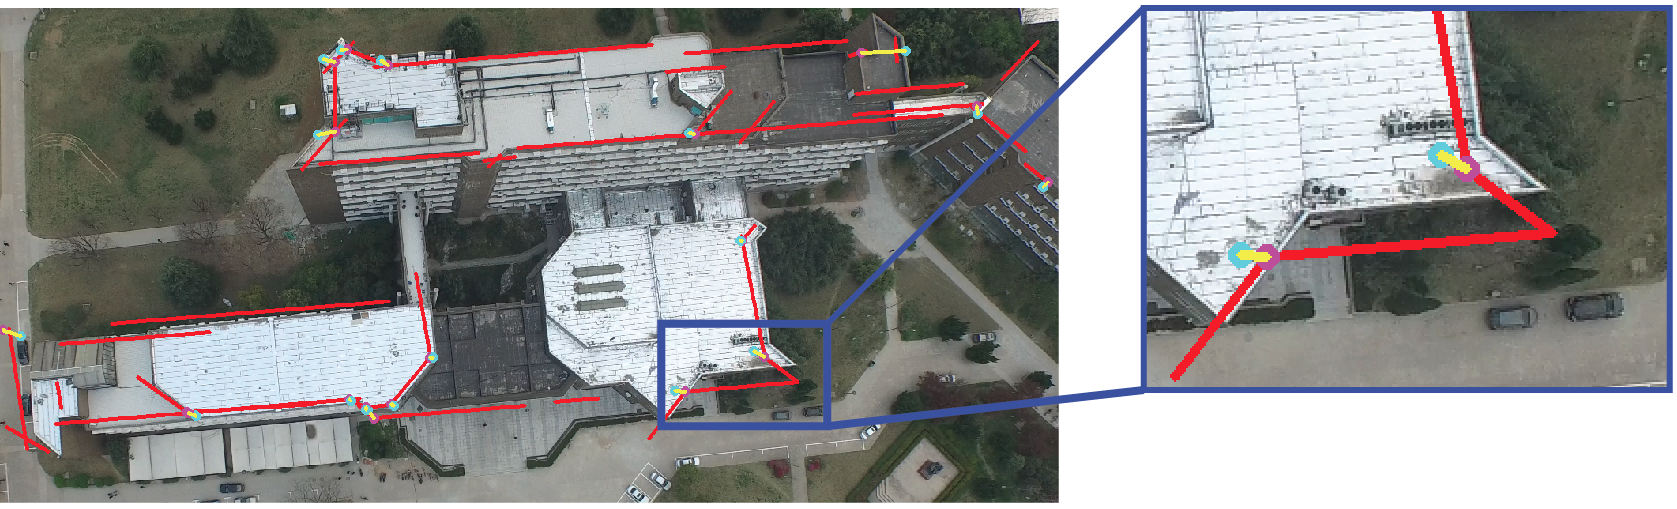
\includegraphics[width=0.5\textwidth]{figures/details_png}
	\caption{Finding paired 3D and 2D feature points: for a 3D feature point, we project it on the overhead image (magenta points) using current project matrix and search in its $k\times k$ neighborhood for a corner (cyan points). These 3D feature points and corresponding corners form pairs of feature points for next iteration of calculating project matrix.}
	\label{fig:overview}
\end{figure}
\section{Our Approach}
Given a building point cloud, we first extract contours of building roofs in different altitudes according to the altitude histogram of points, where each contour is fit into a set of line segments (Figure 1b). And then the contours are matched with the edge map of the overhead image respectively using a shape matching technique of \cite{FDCM}. A local project matrix is achieved for each contour after shape matching (Figure 1c). Note that we need a global project matrix instead of local ones to estimate the camera pose. So we treat the results of shape matching as the initialization of following global optimizing procedure. 

To calculate the global project matrix between the whole point cloud and the overhead image, we need a series of paired 3D feature points and corresponding 2D feature points. We take the intersections of neighboring line segments of the contours as 3D feature points. And then we employ an iterative algorithm to optimize the global project matrix by alternatively finding corresponding 2D feature points and calculating the project matrix, where we utilize the results of shape matching as initial project matrix.

To be more specific, we apply two steps in every iteration alternatively until the convergence. (1)~As shown in Figure~2, for a 3D feature point we project it on the overhead image using current project matrix (magenta points) and search in its $k\times k$ neighborhood for a corner with maximal corner response (cyan points). These 3D feature points and corresponding corners form paired feature points for the next step of calculating project matrix.
%Once a set of paired 3D and 2D feature points is achieved, we randomly select a subset of these feature point pairs to calculate a global matrix. 
(2) With a set of paired 3D and 2D feature points, we can optimize a global project matrix by minimizing the average of distances between projected contours and the edges of the overhead image, which can be accelerated by distance transformation. And the newly calculated project matrix is used for the next iteration of finding paired feature points.

With the optimized global project matrix and pre-calibrated intrinsic matrix of the camera, we can finally estimate the 6 degree-of-freedom camera pose of the overhead image in point cloud coordinate system.
% Be more specific?
\section{Experiments and Future Work}
We tested the proposed approach on a newly collected dataset, which contains several low-altitude overhead images and corresponding building point clouds. Figure 1(d) shows one of the results, where we project roof contours on the overhead image. Since most of the consuming time is spent in the shape matching stage and the optimizing stage is fast, we intend to implement a faster version of the algorithm and extend it to video-based problems. 

\bibliographystyle{ACM-Reference-Format}
\bibliography{Poster_bib} 

\end{document}
